\begin{figure}[htpb]
	\centering\capstart{}
	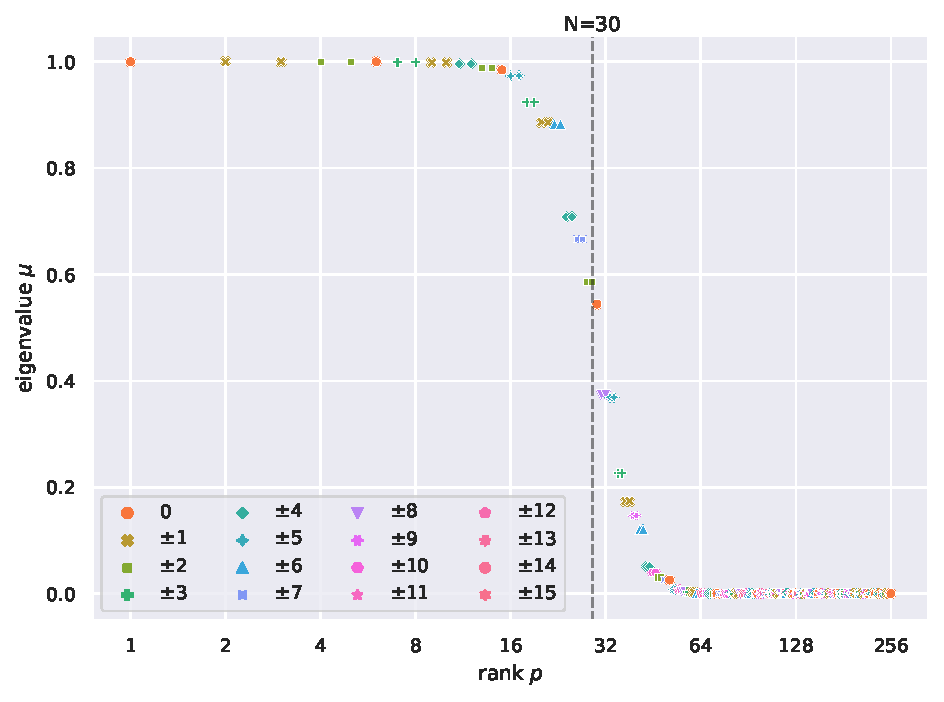
\includegraphics[width=\textwidth]{polar_cap_eigenvalues.pdf}
	\caption[
		The Slepian eigenvalues within a \(\SI{40}{\degree}\) polar cap
	]{
		The ordered Slepian eigenvalues within a polar cap of colatitudinal radius \(\theta_{0}=\SI{40}{\degree}\).
		The bandlimit here is \(L=16\), which corresponds to a Shannon number of \(N=30\), as indicated on the plot.
		Initially, the eigenvalues are \(\almost{\num{1}}\), before decreasing rapidly around the Shannon number, and where the majority of the later eigenvalues are \(\almost{\num{0}}\).
	}\label{fig:chapter2_polar_cap_eigenvalues}
\end{figure}
